\documentclass[smaller]{beamer}
\usetheme[english]{Berlin}
\usepackage{ngerman}
\useoutertheme{infolines}
\beamertemplatenavigationsymbolsempty
\setbeamertemplate{caption}[numbered]
\usepackage{pgfplots,tikz,subfigure}
\usepackage{amsmath,amsthm}
\usepackage{hyperref,graphics,graphicx,color,algorithm,algorithmic,enumerate}
\usepackage{mymacros,wrapfig,relsize}
\usepackage{pict2e}
\usepackage[utf8x]{inputenc}

\newcommand{\ri}{\mathrm{i}}
\newcommand{\T}{\mathsf{T}}
\renewcommand{\H}{\mathsf{H}}
\newcommand{\eps}{\varepsilon}
\newcommand{\To}{\rightarrow}
\newcommand{\sddots}{\scalebox{0.6}{$\ddots$}}
\usepackage[pdf]{pstricks}
\usepackage{sansmathfonts}
\usepackage{eurosym}
\usepackage{ulem}
%\usepackage{arev}
%\renewcommand\familydefault{\sfdefault}

\DeclareMathOperator{\loc}{loc}
\DeclareMathOperator{\rank}{rank}
\DeclareMathOperator{\RE}{Re}
\DeclareMathOperator{\IM}{Im}
\DeclareMathOperator{\In}{In}
\DeclareMathOperator{\im}{im}
\DeclareMathOperator{\Gl}{Gl}
\DeclareMathOperator{\spa}{span}
\DeclareMathOperator{\ext}{{ext}}
\DeclareMathOperator{\ind}{ind}
\DeclareMathOperator{\normalrank}{normalrank}
\DeclareMathOperator{\essup}{ess\,sup}
\DeclareMathOperator{\vect}{vec}

\newcommand{\re}{\mathrm{e}}
\newcommand{\ddt}{\tfrac{\mathrm{d}}{\mathrm{d}t}}
\newcommand{\sys}[4]{\left[\begin{array}{c|c} #1 & #2 \\ \hline #3 & #4 \end{array}\right]}

\renewcommand{\tilde}{\widetilde}
\renewcommand{\hat}{\widehat}


\title[]{Optimierung f\"ur Studierende der Informatik}
\subtitle{-- 9. Vorlesung --}
\author[Matthias Voigt]{\textbf{Matthias Voigt$^{1,2}$}}
\institute[]{
\begin{columns}
%\begin{center}
\column{0.45\textwidth}{\centering {$^1$Universit\"at Hamburg \\ Fachbereich Mathematik \\ Hamburg \\ }}
\column{0.45\textwidth}{\centering {$^2$Technische Universit\"at Berlin \\ Institut f\"ur Mathematik \\ Berlin  \\}}
%\end{center}
\end{columns}
}
\date[]{Universit\"at Hamburg
\begin{columns}
\column{0.45\textwidth}{\centering 
\includegraphics[width = 1.2\textwidth]{uhh-logo.png}\\}
\end{columns}
}

\definecolor{tucgreen}{rgb}{0.0,0.5,0.27}
\definecolor{tucred}{rgb}{0.75,0,0}
\definecolor{tucorange}{rgb}{1.0,.5625,0}
\definecolor{mpired}{HTML}{990000}
\definecolor{mpigreen}{HTML}{5C871D}
\definecolor{mpiblue}{HTML}{006AA9}
\definecolor{mpibg1}{HTML}{5D8B8A}
\definecolor{mpibg2}{HTML}{BFDFDE}
\definecolor{mpibg3}{HTML}{A7C1C0}
\definecolor{mpibg4}{HTML}{7DA9A8}
\definecolor{mpigrey}{rgb}{0.9294,0.9294,0.8784}

\begin{document}

\maketitle

\begin{frame}
\frametitle{Beispiel 2}
Wir betrachten den folgenden bipartiten Graphen $G=(V,E)$:

\begin{center}
 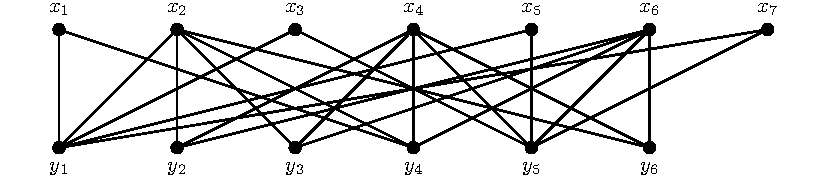
\includegraphics[scale = 0.8]{fig57.pdf}
\end{center}

Es sei $X = \bigl\{ x_1,\ldots,x_7 \bigr\}$ und $Y = \bigl\{ y_1,\ldots,y_6 \bigr\}$. Wie in Beispiel 1 besteht die Aufgabe darin, ein Matching mit maximaler Kantenzahl und gleichzeitig eine minimale Knotenüberdeckung zu finden. \\ \vspace*{0.2cm}

Hierzu soll der Algorithmus von Edmonds und Karp verwendet werden, und auch diesmal soll die Regel ($\star$) angewandt werden, d.h., \alert{stehen mehrere Knoten zur Markierung zur Verfügung, ist zunächst derjenige mit dem kleinsten Index zu markieren.}
\end{frame}

\begin{frame}
\frametitle{Art der Beschreibung}
Im Prinzip wird in Beispiel 2 alles wie in Beispiel 1 ablaufen. \alert{Ein wesentlicher Unterschied besteht jedoch in der Art der Beschreibung}: \\ \vspace*{0.2cm}

Das Netzwerk $N=(G',c,s,t)$ wird nicht mehr erwähnt werden; wir haben es höchstens noch im Hinterkopf. In der folgenden Beschreibung verwenden wir nur noch Ausdrucksweisen, die mit Matchings in bipartiten Graphen zusammenhängen; Ausdrucksweisen, die mit Netzwerken und Flüssen zusammenhängen, werden vermieden.  \alert{Das hat den Vorteil, dass alles einfacher, übersichtlicher und kürzer wird}.
\end{frame}

\begin{frame}
\frametitle{Das Matching $M_5$}
 Mit dem \alert{leeren Matching $M_0 = \emptyset$} geht es los; in der ersten Iteration wählt der Algorithmus die Kante $\big\{ x_1,y_1 \big\}$ als Matchingkante aus. (Dies läuft im Detail wie in Beispiel 1 ab.) Am Ende der 1. Iteration gilt also $M_1 = \big\{ \{x_1,y_1\} \big\}$. \\ \vspace*{0.2cm}
 
 Im Verlauf der 2.-5. Iteration kommen dann -- in der angegebenen Reihenfolge -- die Kanten $\big\{ x_2,y_2 \big\}$, $\big\{ x_3,y_5 \big\}$, $\big\{ x_4,y_3 \big\}$ und $\big\{ x_6,y_4 \big\}$ hinzu.
 
 \alert{Wir können also festhalten:} Nach fünf Iterationen lautet das aktuelle Matching wie folgt (vgl. Zeichnung):
\[
M_5 = \Big\{ 
\big\{ x_1,y_1 \big\}, 
\big\{ x_2,y_2 \big\}, 
\big\{ x_3,y_5 \big\}, 
\big\{ x_4,y_3 \big\},
\big\{ x_6,y_4 \big\}
\Big\}.
\]
\end{frame}

\begin{frame}
 \frametitle{Darstellung von $M_5$ und die 6. Iteration}
 \begin{center}
  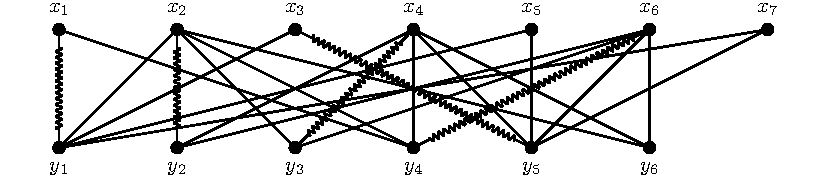
\includegraphics[scale=0.8]{fig58.pdf}
 \end{center}
In der 6. Iteration findet der Algorithmus den augmentierenden Pfad
\[
\big( x_5, y_1, x_1, y_4, x_6, y_6 \big)
\]
und ändert das aktuelle Matching entsprechend ab \alert{(Austausch der Matchingkanten gegen die Nicht-Matchingkanten dieses Pfads):} $\big\{ x_5,y_1 \big\}$, $\big\{ x_1,y_4 \big\}$ und $\big\{ x_6,y_6 \big\}$ werden in die aktuelle Menge der Matchingkanten aufgenommen, $\big\{ x_1,y_1 \big\}$ und $\big\{ x_6,y_4 \big\}$ verlassen diese Menge. Nach der 6. Iteration lautet das aktuelle Matching demnach:
\[
M_6 = \Big\{ 
\big\{ x_1,y_4 \big\}, 
\big\{ x_2,y_2 \big\}, 
\big\{ x_3,y_5 \big\}, 
\big\{ x_4,y_3 \big\},
\big\{ x_5,y_1 \big\},
\big\{ x_6,y_6 \big\}
\Big\}.
\]
\end{frame}

\begin{frame}
 \frametitle{Darstellung von $M_6$ und die 7. Iteration}
 \begin{center}
  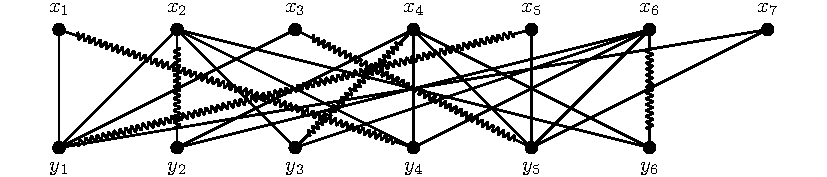
\includegraphics[scale=0.8]{fig59.pdf}
 \end{center}
 In der 7. Iteration versucht der Algorithmus, einen augmentierenden Pfad zu finden, der in $x_7$ startet -- was nicht gelingt. Dabei werden die folgenden Knoten --~in der angegebenen Reihenfolge~-- mit alternierenden Pfaden erreicht und markiert: $$x_7, y_1, y_5, x_5, x_3.$$

\alert{Ergebnis}: Der Algorithmus liefert das obige Matching $M_6$ mit 6 Kanten zusammen mit der minimalen Knotenüberdeckung
\[
U = \big\{ x_1, x_2, x_4, x_6, y_1, y_5 \big\}.
\]

In der nachfolgenden Zeichnung wird dieses Ergebnis veranschaulicht; die Knoten aus $U$ sind durch ein Quadrat gekennzeichnet.
\end{frame}

\begin{frame}
\frametitle{Das Ergebnis}
 \begin{center}
  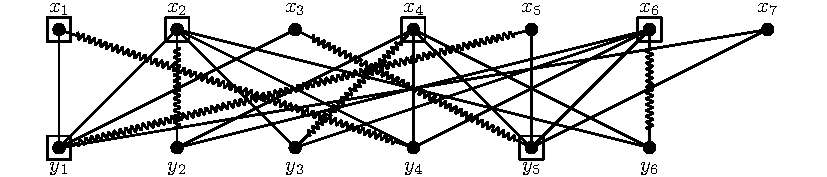
\includegraphics[scale=0.8]{fig60.pdf}
 \end{center}
 \alert{Wie kommt man auf die minimale Knotenüberdeckung $U = \big\{ x_1, x_2, x_4, x_6, y_1, y_5 \big\}$}?

Die Antwort findet sich in Vorlesung 8: Bezeichnen wir (wie dort) mit $S$ die Menge der in der 7. Iteration mittels alternierender Pfade erreichbaren Knoten, so ist
\[
U = \big( X \setminus S \big) \cup \big( Y \cap S \big)
\]
die gewünschte Knotenüberdeckung.
\end{frame}

\begin{frame}
\frametitle{Ausschließlich Begriffe aus der Welt der Matchings}
Wir betonen noch einmal: In der Darstellung von Beispiel 2 wurden keine Begriffe aus der \alert{{\glqq}Welt der Flussnetzwerke{\grqq}} verwendet, sondern nur noch Begriffe aus der \alert{{\glqq}Welt der Matchings{\grqq}}. \\ \vspace*{0.2cm}

Beispielsweise war nicht mehr von zunehmenden Pfaden zu einem Knoten die Rede, sondern es ging um \alert{Erreichbarkeit durch alternierende Pfade}. Dieses Umsteigen auf andere Sprechweisen ist üblich und vor allem auch angemessen: \\ \vspace*{0.2cm}

Es geht ja in der Fragestellung ausschließlich um Matchings in ungerichteten Graphen und nicht um Flüsse in Netzwerken. Ermöglicht wurde das Umsteigen auf andere Sprechweisen durch die Ergebnisse aus Vorlesung 8.
\end{frame}

\begin{frame}
\frametitle{Knotenüberdeckungen in beliebigen Graphen}
Ist $G=(V,E)$ ein \alert{bipartiter} Graph, so wissen wir, wie man in $G$ eine Knotenüberdeckung mit möglichst wenigen Knoten findet: \\ \vspace*{0.2cm}

Wir haben einen Algorithmus mit polynomieller Laufzeit kennengelernt, der
\begin{itemize}
 \item sowohl ein \alert{Matching mit maximaler Kantenzahl};
 \item als auch eine \alert{Knotenüberdeckung mit minimaler Knotenzahl} liefert.
\end{itemize} \vspace*{0.2cm}

Ist $G=(V,E)$ ein \alert{beliebiger}, nicht notwendig bipartiter Graph, so ist die Situation gänzlich anders: \\ \vspace*{0.2cm}

Bei dem Problem, in $G$ eine Knotenüberdeckung mit minimaler Knotenzahl zu finden, handelt es sich um ein \alert{NP-schweres Optimierungsproblem}. Ein Algorithmus mit polynomieller Laufzeit existiert für dieses Problem demnach nur, wenn P $=$ NP gilt, was allgemein als sehr unwahrscheinlich angesehen wird.
\end{frame}

\begin{frame}
\frametitle{$\gamma$-Approximationsalgorithmen}
\textbf{Was tun?} Eine Möglichkeit ist, nach einem \alert{Approximationsalgorithmus} Ausschau zu halten, d.h. nach einem Algorithmus mit polynomieller Laufzeit, der eine \alert{Näherungslösung mit Gütegarantie} liefert. Einen solchen Algorithmus werden wir im Folgenden kennenlernen. \\ \vspace*{0.2cm}
Es sei $\gamma \geq 1$ eine reelle Zahl. Bevor wir auf das Knotenüberdeckungsproblem zu sprechen kommen, soll definiert werden, was unter einer \structure{Näherungslösung mit Gütegarantie} $\gamma$ und unter einem \structure{$\gamma$-Approximations\-algorithmus} zu verstehen ist. \\ \vspace*{0.2cm}
Zu diesem Zweck nehmen wir an, dass ein \alert{Minimierungsproblem} vorliegt, für Maximierungsprobleme trifft man ähnliche Definitionen und verwendet ähnliche Sprechweisen.
\end{frame}

\begin{frame}
\frametitle{Näherungslösungen mit Gütegarantie}
Wir setzen voraus, dass das Problem eine optimale Lösung besitzt. \alert{Mit $L^*$ sei der (unbekannte) optimale Zielfunktionswert bezeichnet}. \\ \vspace*{0.2cm} 

\textbf{Außerdem:} $\mathcal{A}$ sei ein Algorithmus für das vorliegende Problem, der eine Lösung liefert, die nicht notwendigerweise optimal ist. \alert{Der Wert der von $\mathcal{A}$ gelieferten Lösung sei mit $L_{\mathcal{A}}$ bezeichnet}. \\ \vspace*{0.2cm}

\textbf{Definition:} Man sagt, dass $\mathcal{A}$ eine \structure{Näherungslösung mit Gütegarantie} $\gamma$ liefert, falls stets (d.h. für alle Instanzen des betrachteten Problems) gilt:
\begin{equation}
\label{eq:11:4}
L_{\mathcal{A}} \leq \gamma L^*.
\end{equation}

Die Ungleichung \eqref{eq:11:4} bedeutet, dass der Wert der von $\mathcal{A}$ gelieferten Lösung niemals schlechter als das $\gamma$-fache des Optimalwerts $L^*$ ist. Gilt zusätzlich zu \eqref{eq:11:4}, dass es sich bei $\mathcal{A}$ um einen polynomiellen Algorithmus handelt, so spricht man von einem \structure{$\gamma$-Approximationsalgorithmus}.
\end{frame}

\begin{frame}
\frametitle{Die Rolle unterer Schranken}
Liegt ein polynomieller Algorithmus $\mathcal{A}$ vor, von dem man nachweisen möchte, dass es sich für ein bestimmtes $\gamma \geq 1$ um einen $\gamma$-Approximationsalgorithmus handelt, \alert{so steht man vor der Schwierigkeit, dass $L^*$ unbekannt ist}. \\ \vspace*{0.2cm}

Es stellt sich die Frage, wie man \eqref{eq:11:4} nachweisen kann, wenn man $L^*$ gar nicht kennt. Die entscheidende Rolle hierbei spielen \alert{untere Schranken} für $L^*$: Der Wert $L^*$ ist zwar unbekannt, aber häufig kennt man eine untere Schranke $B$ für $L^*$, d.h., man kennt eine Größe $B$, für die gilt:
\begin{equation}
\label{eq:11:5}
B \leq L^*.
\end{equation}

Gelingt es einem nun nachzuweisen, dass
\begin{equation}
\label{eq:11:6}
L_{\mathcal{A}} \leq \gamma B,
\end{equation}

gilt, so erhält man wegen $B \leq L^*$, dass (\ref{eq:11:4}) erfüllt ist:
\[
L_{\mathcal{A}} \leq \gamma B \leq \gamma L^*.
\]
\end{frame}

\begin{frame}
\frametitle{Was ist zu tun?}
Man hat also Zweierlei zu tun, um zu \eqref{eq:11:4} zu gelangen:
\begin{itemize}
\item Erstens ist eine geeignete untere Schranke $B$ zu finden;
\item zweitens ist für diese Schranke \eqref{eq:11:6} nachzuweisen.
\end{itemize}

Im Folgenden demonstrieren wir die geschilderte Vorgehensweise anhand des \alert{Knotenüberdeckungsproblems}. Dies lässt sich wie folgt formulieren.
\end{frame}

\begin{frame}
\frametitle{Das Knotenüberdeckungsproblem}
\textbf{Eingabe}: ein Graph $G=(V,E)$, \\ \vspace*{0.2cm}
\textbf{Gesucht}: eine Knotenüberdeckung von $G$ mit minimaler Knotenzahl. \\ \vspace*{0.2cm}

Anders gesagt: Es ist nach einer Knotenüberdeckung $U$ von $G$ mit $|U| = c(G)$ gefragt. Zur Definition der \structure{Knotenüberdeckungszahl} $c(G)$ siehe Vorlesung 8. Es sei noch einmal betont:
\begin{itemize}
\item Wir können nicht erwarten, einen polynomiellen Algorithmus zur exakten Lösung des Knotenüberdeckungsproblems zu finden, da es sich um ein NP-schweres Optimierungsproblem handelt.
\item Aus diesem Grund halten wir nach einem $\gamma$-Approximationsalgorithmus Ausschau, wobei wir uns wünschen, dass $\gamma$ {\glqq}nicht allzu groß{\grqq} ist.
\end{itemize}
\end{frame}

\begin{frame}
\frametitle{Nicht erweiterbare Matchings}
Es wird ein 2-Approximationsalgorithmus für das Knotenüberdeckungsproblem vorgestellt werden. Hierzu benötigen wir den Begriff eines \structure{nicht erweiterbaren} Matchings, der wie folgt definiert wird: \\ \vspace*{0.2cm}

\textbf{Definition:} Es sei $G=(V,E)$ ein Graph. Ein Matching $M$ von $G$ wird \structure{nicht erweiterbar} genannt, wenn es maximal in Bezug auf die Inklusion $\subseteq$ ist, d.h., wenn es unmöglich ist, $M$ durch Hinzunahme einer weiteren Kante $e \in E$ zu einem größeren Matching von $G$ zu erweitern. \\ \vspace*{0.2cm}

Es ist sorgfältig zwischen den Begriffen \alert{nicht erweiterbares Matching} und \alert{Matching mit maximaler Kantenzahl} zu unterscheiden. \\ \vspace*{0.2cm}

Als \textbf{Beispiel} betrachten wir den folgenden Graph:
\end{frame}

\begin{frame}
\frametitle{Ein Beispiel}
\begin{center}
 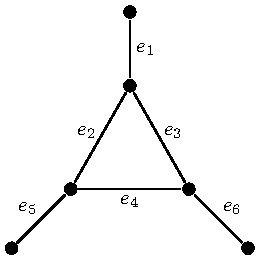
\includegraphics{fig61.pdf}
\end{center}

In diesem Graph ist die Menge $M = \big\{ e_1,e_4 \big\}$ ein nicht erweiterbares Matching, das aber keineswegs maximale Kantenzahl besitzt; $M' = \big\{ e_1,e_5,e_6 \big\}$ besitzt dagegen maximale Kantenzahl.
\end{frame}

\begin{frame}
\frametitle{Bestimmung eines nicht erweiterbaren Matchings}
Für einen gegebenen Graphen $G=(V,E)$ ein nicht erweiterbares Matching zu finden, ist sehr leicht: \\ \vspace*{0.2cm} 
\begin{itemize}
 \item Man beginnt mit dem leeren Matching $M = \emptyset$ und geht die Kanten von $G$ in einer beliebigen Reihenfolge durch. 
 \item Stößt man dabei auf eine Kante $e$, durch deren Hinzunahme das aktuelle Matching $M$ zu einem größeren Matching wird, so nehme man $e$ in $M$ auf; andernfalls wird $e$ nicht aufgenommen.
\end{itemize}

Hieran anknüpfend erhält man den gewünschten \alert{Approximationsalgorithmus für das Knotenüberdeckungsproblem:} \\ \vspace*{0.2cm}

\alert{Bestimme ein nicht erweiterbares Matching $M$ von $G$ und wähle als Output $U$ die Menge aller Knoten, die mit einer Kante von $M$ inzidieren.}
\end{frame}

\begin{frame}
\frametitle{Ein 2-Approximationsalgorithmus}
\textbf{Satz:} Der beschriebene Algorithmus ist ein 2-Approximationsalgorithmus für das Knotenüberdeckungsproblem. \\ \vspace*{0.2cm}
\textbf{Beweis:} Es handelt sich um einen \alert{polynomiellen Algorithmus}, da ein nicht erweiterbares Matching $M$ (wie zuvor beschrieben) in polynomieller Zeit gefunden werden kann. \\ \vspace*{0.2cm}

\alert{Das vom Algorithmus gelieferte $U$ ist eine Knotenüberdeckung:} Würde $U$ eine Kante $e$ von $G$ nicht treffen, so könnte man $e$ zu $M$ hinzunehmen, d.h., $M$ wäre erweiterbar. Es bleibt zu zeigen:
\begin{equation}
\label{eq:11:7}
|U| \leq 2c(G).
\end{equation}

Die Rolle der unteren Schranke $B$ aus \eqref{eq:11:5} wird von $|M|$ übernommen: Es gilt $|M| \leq c(G)$, da eine Knotenüberdeckung alle Kanten aus $M$ treffen muss. Es folgt $2|M| \leq 2c(G)$, woraus man wegen $|U|=2|M|$ die gewünschte Ungleichung \eqref{eq:11:7} erhält. \qquad $\Box$
\end{frame}

\begin{frame}
\frametitle{Verbesserung der Knotenüberdeckung}
\textbf{Frage}: Ist es möglich, den gefundenen Faktor 2 zu verbessern, indem man den Algorithmus unverändert lässt, aber eine raffiniertere Analyse des Algorithmus vornimmt? \\ \vspace*{0.2cm}

\textbf{Antwort}: Dass dies nicht möglich ist, erkennt man anhand des vollständig bipartiten Graphen $K_{n,n}$. \\ \vspace*{0.2cm}

\textbf{Definition:} 
\begin{enumerate}[a)]
\item Ein bipartiter Graph $G = (V,E)$ heißt \structure{vollständig bipartit}, falls Folgendes gilt: $V$ zerfällt in zwei disjunkten Mengen $X$ und $Y$, und $E$ besteht aus sämtlichen Kanten $\{x, y\}$ mit $x \in X$ und $y \in Y$. 
\item Gilt in a) $|X| = |Y| = n$, so bezeichnet man den vollständig bipartiten Graphen aus a) mit \structure{$K_{n,n}$}.
\end{enumerate}
\end{frame}

\begin{frame}
\frametitle{Verbesserung der Knotenüberdeckung}
\textbf{Nächste Frage}: Gibt es einen $\gamma$-Approximationsalgorithmus für das Knotenüberdeckungsproblem für ein $\gamma < 2$? \\ \vspace*{0.2cm}

\textbf{Antwort}: Das ist nicht bekannt. Es handelt sich um ein berühmtes offenes Problem. \\ \vspace*{0.2cm}

Bekannt ist jedoch Folgendes: \\ \vspace*{0.2cm}

\textbf{Satz (Dinur und Safra 2001):}
Falls P $\neq$ NP, so existiert kein $\gamma$-Approximationsalgorithmus für das Knotenüberdeckungsproblem für $\gamma < 1.3606$.
\end{frame}

\begin{frame}
\frametitle{Gewichtete Knotenüberdeckungen}
Es sei ein Graph $G=(V,E)$ gegeben, wobei wir $V = \big\{ 1,\ldots,n \big\}$ annehmen. Jeder Knoten $i$ besitzt ein \structure{Gewicht} $w_i \geq 0$ mit $w_i \in \mathbb{Q}$ ($i=1,\ldots,n$). \\ \vspace*{0.2cm}

Zu finden ist eine Knotenüberdeckung $U \subseteq V$ mit möglichst kleinem Gewicht, wobei das Gewicht von $U$ definiert wird durch
\[
w(U) = \sum\limits_{i \in U}{w_i}.
\]

Sind alle Gewichte gleich 1, so liegt der ursprünglich betrachtete Fall vor, in dem die Anzahl der Knoten in einer Knotenüberdeckung zu minimieren ist. Das ursprünglich betrachtete Problem ist also ein Spezialfall des allgemeinen gewichteten Problems.
\end{frame}

\begin{frame}
\frametitle{Ein ganzzahliges lineares Optimierungsproblem}
Das gewichtete Knotenüberdeckungsproblem lässt sich wie folgt als ein \alert{ganzzahliges lineares Optimierungsproblem} schreiben, das wir mit (ILP) bezeichnen:
\begin{align}
\tag{ILP}
\begin{alignedat}{5}
& \text{minimiere } & \rlap{$w_1x_1 + \ldots + w_nx_n$} & & & & & \\
& \rlap{unter den Nebenbedingungen} & & & & & & \\
&&\ x_i &\ + &\ x_j &\ \geq &\ 1, & \qquad \big\{ i,j \big\} \in E, \\
&& & & & & \llap{$x_i \in \big\{ 0,1 \big\},$}  & \qquad i \in V.
\end{alignedat}
\end{align}
\end{frame}

\begin{frame}
\frametitle{Interpretation}
Jedem Knoten $i$ entspricht hierbei eine Variable $x_i$. Außerdem entspricht jeder zulässigen Lösung $x = (x_1,\ldots,x_n)$ von (ILP) eine Knotenüberdeckung $U$, wenn man die folgende (naheliegende) \alert{Interpretation} vornimmt:
\begin{itemize}
 \item $x_i=1$ bedeutet, dass der Knoten $i$ in $U$ liegt,
 \item $x_i=0$ ist gleichbedeutend mit $i \notin U$.
\end{itemize}
\textbf{Man beachte:} Für jede Kante $\big\{ i,j \big\}$ wird durch die Bedingung $x_i+x_j \geq 1$ gesichert, dass $i \in U$ oder $j \in U$ gilt. \\ \vspace*{0.2cm}

Umgekehrt erhält man auf entsprechende Art zu jeder Knotenüberdeckung $U$ eine zulässige Lösung von (ILP). 
\end{frame}

\begin{frame}
\frametitle{Zwei Feststellungen}
Zusammenfassend können wir feststellen:\\ \vspace*{0.2cm}
\textbf{Feststellung:}
Ist $x = (x_1,\ldots,x_n)$ eine \alert{zulässige Lösung dieses ganzzahligen linearen Programmierungsproblems}, so ist $U = \big\{ i \in V : x_i = 1 \big\}$ \alert{eine Knotenüberdeckung} (und umgekehrt entspricht auch jeder Knotenüberdeckung eine zulässige Lösung von (ILP)). \\ \vspace*{0.2cm}

Außerdem gilt: \\ \vspace*{0.2cm}

\textbf{Feststellung:}
Ist $x^* = (x_1^*,\ldots,x_n^*)$ eine \alert{optimale Lösung des ganzzahligen linearen Programmierungsproblems (ILP)}, so ist $U^* = \bigl\{ i \in V : x_i^* = 1 \bigr\}$ eine \alert{minimale Knotenüberdeckung (und umgekehrt)}, wobei minimale Knotenüberdeckung bedeuten soll: Knotenüberdeckung minimalen Gewichts.
\end{frame}

\begin{frame}
\frametitle{Relaxieren und Runden}
 Im vorangegangenen Abschnitt haben wir das gewichtete Knotenüberdeckungsproblem in ein \alert{ganzzahliges lineares Optimierungsproblem (ILP)} umgeschrieben. Dies ermöglicht uns, die \alert{LP-Relaxation} des Problems zu betrachten:
\begin{align}
\tag{LP}
\begin{alignedat}{5}
& \text{minimiere } & \rlap{$w_1x_1 + \ldots + w_nx_n$} & & & & & \\
& \rlap{unter den Nebenbedingungen} & & & & & & \\
&&\ x_i &\ + &\ x_j &\ \geq &\ 1, & \qquad \bigl\{ i,j \bigr\} \in E, \\
&&\     &\   &\  &\  &\ \llap{$0 \leq x_i \leq 1,$} & \qquad i \in V. \\
\end{alignedat}
\end{align}

\textbf{Beobachtung:} Es gilt
\begin{equation}
\label{eq:11:8}
\alert{\text{Optimalwert von (LP)} \leq \text{Optimalwert von (ILP)}.}
\end{equation}

\textbf{Denn:} Jede zulässige Lösung von (ILP) ist auch eine zulässige Lösung von (LP).
\end{frame}

\begin{frame}
 \frametitle{Optimalwert von (LP) vs. Optimalwert von (ILP)}
  Das folgende \textbf{Beispiel} zeigt, dass
  \begin{equation*}
    \alert{\text{Optimalwert von (LP)} < \text{Optimalwert von (ILP)}}
   \end{equation*}
   möglich ist: \\ \vspace*{0.2cm}
  
  Es sei $G=(V,E)$ mit $V = \big\{ 1,2,3 \big\}$ und $E = \big\{ \{ 1,2\}, \{2,3\}, \{3,1\} \big\}$. Alle Gewichte seien gleich 1, d.h. $w_1=w_2=w_3=1$. Der Optimalwert von (ILP) ist offenbar gleich 2. \\ \vspace*{0.2cm}
  
  Für (LP) gibt es dagegen eine zulässige Lösung mit Zielfunktionswert $\frac{3}{2}$: Man braucht nur $x_1 = x_2 = x_3 = \frac{1}{2}$ zu wählen (siehe Zeichnung).

\begin{center}
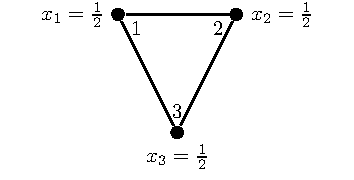
\includegraphics{fig62.pdf}
\end{center}
\end{frame}

\begin{frame}
\frametitle{Relaxieren und Runden}
Die Methode, die zum Einsatz kommen wird, lässt sich wie folgt beschreiben:

\begin{center}
\alert{Man löst die LP-Relaxation und rundet.}
\end{center}

\textbf{Genauer:} Es sei $x^* = (x_1^*,\ldots,x_n^*)$ eine optimale Lösung der LP-Relaxation (LP). Dann betrachten wir die Menge $U \subseteq V$, die wie folgt definiert ist:
\[
U = \left\{ i \in V : x_i^* \geq \frac{1}{2} \right\}.
\]

\textbf{Satz:} Es sei $x^* = (x_1^*,\ldots,x_n^*)$ eine optimale Lösung der LP-Relaxation (LP) des gewichteten Knotenüberdeckungsproblems (ILP). Dann ist $U = \big\{ i \in V : x_i^* \geq \frac{1}{2} \big\}$ eine Knotenüberdeckung mit einem Gewicht $w(U)$, das \alert{höchstens doppelt so groß} ist wie das Gewicht einer minimalen Knotenüberdeckung.
\end{frame}

\begin{frame}
\frametitle{Beweis des Satzes}
\textbf{Beweis:} Wir weisen zunächst nach, dass die Menge $U = \big\{ i \in V : x_i^* \geq \frac{1}{2} \big\}$ tatsächlich eine Knotenüberdeckung ist. Zu diesem Zweck betrachten wir eine beliebige Kante $e = \big\{ i,j \big\} \in E$. \\ \vspace*{0.2cm}

Da $(x_1^*, \ldots, x_n^*)$ eine Lösung von (LP) ist, gilt $x_i^* + x_j^* \geq 1$. Deshalb muss $x_i^* \geq \frac{1}{2}$ oder $x_j^* \geq \frac{1}{2}$ (oder beides) gelten. Es folgt, dass $i \in U$ oder $j \in U$ erfüllt ist, d.h., \alert{$U$ ist eine Knotenüberdeckung}. \\ \vspace*{0.2cm}

Es bleibt zu zeigen: $$w(U) = \sum_{i \in U}{w_i}$$ ist höchstens doppelt so groß wie das minimale Gewicht einer Knotenüberdeckung. Dies ergibt sich wie folgt.

\end{frame}

\begin{frame}
\frametitle{Beweis des Satzes}
Es sei $U_{\text{min}}$ eine Knotenüberdeckung minimalen Gewichts. Die Rolle der unteren Schranke $B$ aus (\ref{eq:11:5}) wird in diesem Fall vom Zielfunktionswert $\sum\limits_{i=1}^{n}{w_ix_i^*}$ der optimalen Lösung $x^* = (x_1^*,\ldots,x_n^*)$ von (LP) übernommen. Es gilt nämlich 
\begin{equation}
\label{eq:11:9}
\sum\limits_{i=1}^{n}{w_ix_i^*} \leq w \left( U_{\text{min}} \right).
\end{equation}

Zum Nachweis von (\ref{eq:11:9}) ist nur zu beachten, dass $w\left(U_{\text{min}} \right) = \sum\limits_{i \in U_{\text{min}}}{w_i}$ Zielfunktionswert einer optimalen Lösung von (ILP) ist, nämlich der Lösung $x=(x_1,\ldots,x_n)$ mit
\[
x_i = \begin{cases}
1 & \text{falls } i \in U_{\text{min}} \\
0 & \text{sonst}.
\end{cases}
\]
\end{frame}

\begin{frame}
\frametitle{Beweis des Satzes}
Also: \eqref{eq:11:9} gilt aufgrund der Beobachtung \eqref{eq:11:8}. \\ \vspace*{0.2cm}

Außerdem gilt
\begin{equation}
\label{eq:11:10}
\sum\limits_{i=1}^{n}{w_ix_i^*} \geq \sum\limits_{i \in U}{w_ix_i^*} \stackrel{(\star)}{\geq} \frac{1}{2} \sum\limits_{i \in U}{w_i} = \frac{1}{2}w(U),
\end{equation}

wobei sich die mit $(\star)$ gekennzeichnete Ungleichung von (\ref{eq:11:10}) aus der Tatsache ergibt, dass $x_i^* \geq \frac{1}{2}$ für alle $i \in U$ gilt. \\ \vspace*{0.2cm}

Aus \eqref{eq:11:9} und \eqref{eq:11:10} ergibt sich, dass wie behauptet
\[
w(U) \leq 2w\left(U_{\text{min}}\right)
\]
gilt. \qquad $\Box$
\end{frame}

\begin{frame}
\frametitle{Relaxieren und Runden}
Den Inhalt des vorangegangenen Satzes können wir auch so aussprechen: \\ \vspace*{0.2cm}

\alert{Der Algorithmus {\glqq}Lösen der LP-Relaxation und Runden{\grqq} ist ein 2-Approximationsalgorithmus für das gewichtete Knotenüberdeckungsproblem}. \\ \vspace*{0.2cm}

\textbf{Man beachte:} (LP) lässt sich in \alert{polynomieller Zeit} lösen.
\end{frame}

\begin{frame}
\frametitle{Ähnlichkeiten zwischen Labelling- und Simplexalgorithmus}
Man kann viele Ähnlichkeiten zwischen dem Labelling-Algorithmus und dem Simplexalgorithmus beobachten, beispielsweise diese: Am Schluss, wenn keine Verbesserung mehr möglich ist, erhält man in beiden Fällen eine \alert{Zugabe}; genauer gilt: 
\begin{itemize}
\item Beim \alert{Simplexalgorithmus} erhält man zusätzlich eine \alert{optimale Lösung des dualen Problems};
\item Beim \alert{Labelling-Algorithmus} erhält man neben einem maximalen Fluss auch einen \alert{minimalen Schnitt}.
\end{itemize}
Diese Ähnlichkeiten hängen natürlich damit zusammen, \alert{dass man das Problem, einen maximalen Fluss in einem Netzwerk zu finden, als ein LP-Problem formulieren kann}.
\end{frame}

\begin{frame}
\frametitle{Ein Beispiel}
Zum Einstieg betrachten wir ein weiteres Beispiel:

\begin{center}
 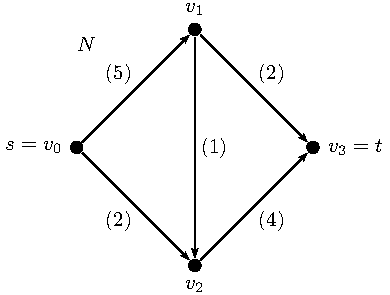
\includegraphics{fig63.pdf}
\end{center}

\end{frame}

\begin{frame}
\frametitle{Einführung von Variablen}
Die geklammerten Zahlen an den Kanten bezeichnen die Kapazitäten. \alert{Für jede Kante führen wir eine Variable ein, die die Stärke des Flusses durch diese Kante angibt}: Führt die Kante $e$ von $v_i$ nach $v_j$, so bezeichnen wir die dazugehörige Variable mit $x_{ij}$. \\ \vspace*{0.2cm}

Im obigen Beispiel haben wir es also mit den folgenden Variablen zu tun:
\[
x_{01},\quad
x_{02},\quad
x_{12},\quad
x_{13},\quad
x_{23}.
\]
\end{frame}

\begin{frame}
\frametitle{Das primale Problem (P)}
Das dazugehörige LP-Problem -- wir wollen es (P) nennen -- lautet:
\begin{align*}
\begin{alignedat}{7}
& \text{maximiere } & x_{01} &\ + &\ x_{02} & & & & & & & &  \\
& \rlap{unter den Nebenbedingungen} & & & & & & & & & & & \\
&& x_{01} &\   &\        &\ - &\ x_{12} &\ - &\ x_{13} &\   &\        &\    = &\ 0,\ \\
&&        &\   &\ x_{02} &\ + &\ x_{12} &\   &\        &\ - &\ x_{23} &\    = &\ 0,\ \\
&& x_{01} &\   &\        &\   &\        &\   &\        &\   &\        &\ \leq &\ 5,\ \\
&&        &\   &\ x_{02} &\   &\        &\   &\        &\   &\        &\ \leq &\ 2,\ \\
&&        &\   &\        &\   &\ x_{12} &\   &\        &\   &\        &\ \leq &\ 1,\ \\
&&        &\   &\        &\   &\        &\   &\ x_{13} &\   &\        &\ \leq &\ 2,\ \\
&&        &\   &\        &\   &\        &\   &\        &\   &\ x_{23} &\ \leq &\ 4,\ \\
&& & & & & & & & & \llap{$x_{01},\ldots,x_{23}$} &\ \geq &\ 0.\
\end{alignedat}
\end{align*}
\end{frame}

\begin{frame}
\frametitle{Aufstellung des dualen Problems}
Wir stellen außerdem das \alert{duale Problem} (D) hierzu auf. \\ \vspace*{0.2cm}

Die ersten beiden Nebenbedingungen von (P) beziehen sich auf die inneren Knoten $v_1$ und $v_2$; die dazugehörigen dualen Variablen wollen wir $y_1$ und $y_2$ nennen. Es handelt sich um freie Variablen, da die ersten beiden Nebenbedingungen von (P) Gleichungen sind. \\ \vspace*{0.2cm}

Die anschließenden fünf Ungleichungen von (P) beziehen sich auf die fünf Kanten von $N$. Die dazugehörigen dualen Variablen wollen wir $y_{01}$, $y_{02}$, $y_{12}$, $y_{13}$ und $y_{23}$ nennen.
\end{frame}

\begin{frame}
\frametitle{Das duale Problem (D)}
Das duale Problem (D) lautet wie folgt:
\begin{align*}
\begin{alignedat}{9}
& \text{minimiere } & & & & &\ 5y_{01} &\ + &\ 2y_{02} &\ + &\ y_{12} &\ + &\ 2y_{13} &\ + &\ 4y_{23} & & \\
& \rlap{unter den Nebenbedingungen} & & & & & & & & & & & & & & & \\
&&  y_1 &\   &\     &\ + &\ y_{01} &\   &\        &\   &\        &\   &\        &\   &\        &\ \geq &\ 1,\ \\
&&      &\   &\ y_2 &\   &\        &\ + &\ y_{02} &\   &\        &\   &\        &\   &\        &\ \geq &\ 1,\ \\
&& -y_1 &\ + &\ y_2 &\   &\        &\   &\        &\ + &\ y_{12} &\   &\        &\   &\        &\ \geq &\ 0,\ \\
&& -y_1 &\   &\     &\   &\        &\   &\        &\   &\        &\ + &\ y_{13} &\   &\        &\ \geq &\ 0,\ \\
&&      &\ - &\ y_2 &\   &\        &\   &\        &\   &\        &\   &\        &\ + &\ y_{23} &\ \geq &\ 0,\ \\
&&     & & & & & & & & & & & & \llap{$y_{01},\ldots,y_{23}$} &\ \geq &\ 0.\
\end{alignedat}
\end{align*}
\end{frame}

\begin{frame}
\frametitle{Das primale Problem (Max-Flow)}
Nachdem wir geade anhand eines Beispiels gesehen haben, wie man zu (P) und (D) gelangt, \alert{wollen wir nun für ein beliebiges Flussnetzwerk $N = (G,c,s,t)$ mit $G = (V,E)$ das Entsprechende durchführen}. \\ \vspace*{0.2cm}

Zu diesem Zweck benennen wir zunächst die Knoten von $N$ wie folgt:
\begin{itemize}
\item $v_0$ sei die Quelle, d.h., $v_0=s$;
\item $v_1,\ldots,v_n$ seien die inneren Knoten;
\item $v_{n+1}$ sei die Senke, d.h., $v_{n+1}=t$.
\end{itemize} \vspace*{0.2cm}

Für jede Kante $(v_i,v_j)$ führen wir eine Variable $x_{ij}$ ein; die Kapazität der Kante $(v_i,v_j)$ sei mit $c_{ij}$ bezeichnet. Es folgt die \alert{Beschreibung von (P)}:
\end{frame}

\begin{frame}
\frametitle{Beschreibung von (P)}
\textbf{Zielfunktion:} maximiere $\displaystyle\sum\limits_{(v_0,v_j) \in E}{x_{0j}}$, \\ \vspace*{0.2cm}

\textbf{Nebenbedingungen}:
\begin{enumerate}[a)]
\item Für jeden inneren Knoten $v_i$ gibt es eine Nebenbedingung, die wie folgt lautet\footnote{Man beachte: In (\ref{eq:10:1}) ist der Index $i$ fest gewählt. Die Formel besagt, dass in $v_i$ ebenso viel hinein wie hinaus fließt.}:
\begin{equation}
\label{eq:10:1}
\sum\limits_{(v_j,v_i) \in E}{x_{ji}} - \sum\limits_{(v_i,v_j) \in E}{x_{ij}} = 0.
\end{equation}

\item Für jede Kante $(v_i,v_j) \in E$ gibt es die Nebenbedingung $x_{ij} \leq c_{ij}$.
\item Für jede Variable $x_{ij}$ gilt die Nichtnegativitätsbedingung $x_{ij} \geq 0$.
\end{enumerate}
\end{frame}

\begin{frame}
\frametitle{Knoten- und Kapazitätsbedingungen}
Damit ist (P) aufgestellt. Es gibt in (P) also -- abgesehen von den Nichtnegativitätsbedingungen -- zwei Typen von Nebenbedingungen:
\begin{enumerate}[a)]
\item die \alert{Knotenbedingungen},
\item die \alert{Kapazitätsbedingungen}.
\end{enumerate} \vspace*{0.2cm}

Durch die Aufstellung von (P) haben wir gesehen, \alert{dass man das Problem, einen maximalen Fluss in einem Netzwerk zu finden, als ein LP-Problem formulieren kann}. \\ \vspace*{0.2cm}

\textbf{Feststellung 1:}
Beim Maximalflussproblem handelt es sich um ein spezielles LP-Problem.
\end{frame}

\begin{frame}
\frametitle{Das duale Problem (Min-Cut)}
Nun wenden wir das \alert{Dualisierungsrezept} auf das Problem (P) an: \\ \vspace*{0.2cm}
Zu jedem inneren Knoten $v_i$ gehört dann eine duale Variable $y_i$, und zu jeder Kante $(v_i,v_j) \in E$ haben wir eine duale Variable $y_{ij}$. Unter Benutzung dieser Bezeichnungen stellen wir im Folgenden das duale Problem (D) auf. \\ \vspace*{0.2cm}

Dabei wird sich herausstellen, dass es einen sehr engen Zusammenhang zwischen minimalen Schnitten $(S,T)$ von $N$ und optimalen Lösungen von (D) gibt. \\ \vspace*{0.2cm}

Die Details der Rechnung finden sich im Skript, wir geben hier nur das \alert{Ergebnis} an:
\end{frame}

\begin{frame}
\frametitle{Das Ergebnis}
\begin{center}
 \alert{Zu jedem minimalen Schnitt $(S,T)$ gehört eine optimale Lösung von (D), die man auf einfache Art aus $(S,T)$ erhält.}
\end{center}
Wir wollen uns anhand unseres einführenden Beispiels anschauen, wie
man aus einem minimalen Schnitt $(S,T)$ eine optimale Lösung von (D) erhält. \\ \vspace*{0.2cm}
Auf der folgenden Folie ist ein maximaler Fluss $f$ und ein minimaler Schnitt
$(S, T)$ für dieses Beispiel angegeben (Wie man $f$ und $(S,T)$ ermitteln kann,
haben wir ja bereits besprochen!):
\end{frame}

\begin{frame}
\frametitle{Ein maximaler Fluss und ein minimaler Schnitt}

\begin{center}
 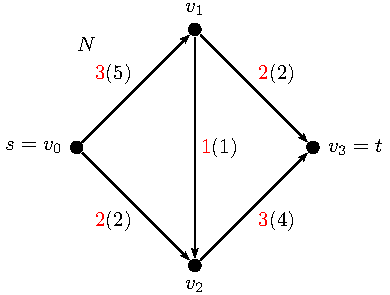
\includegraphics{fig64.pdf}
\end{center}

\begin{itemize}
 \item Ein \alert{maximaler Fluss $f$:} wie in der Zeichnung \alert{rot} angegeben.
 \item Ein \alert{minimaler Schnitt:} $(S, T)$ mit $S = \{s, v_1\}$ und $T = \{v_2, t\}$.
\end{itemize}
Es gilt $w(f) = 5 = c(S,T)$, woran man erkennt, dass tatsächlich ein
maximaler Fluss und ein minimaler Schnitt vorliegt.
\end{frame}

\begin{frame}
\frametitle{Die optimale Lösung von (D)}
Ist ein minimaler Schnitt $(S, T)$ gefunden, so erhält man wie folgt eine
\alert{optimale Lösung von (D)}, die zu $(S, T)$ gehört:
\begin{itemize}
 \item Die dualen Variablen $y_i$, die zu inneren Knoten aus $S$ gehören, werden
auf 1 gesetzt.
 \item Die Variablen $y_{ij}$, die zu Kanten gehören, die von $S$ nach $T$ gehen,
werden ebenfalls auf 1 gesetzt.
 \item Die übrigen Variablen werden auf 0 gesetzt.
\end{itemize} \vspace*{0.2cm}
Im Skript wird nachgewiesen, dass man auf diese Art immer eine optimale
Lösung von (D) erhält. \\ \vspace*{0.2cm}
Für unser \textbf{Beispiel} $S = \{s, v_1\}$ und $T = \{v_2, t\}$ bedeutet dies:
\begin{equation} \tag{$\star$}
y_1 = 1, \quad y_2 = 0, \quad y_{01} = 0, \quad y_{02} = 1, \quad y_{12} = 1, \quad  y_{13} = 1, \quad y_{23} = 0.
\end{equation}
\end{frame}

\begin{frame}
\frametitle{Eine Aufgabe und eine Anmerkung zum allgemeinen Fall}
\textbf{Aufgabe:} Überprüfen Sie, dass es sich bei ($\star$) tatsächlich um eine optimale
Lösung von (D) handelt! \\ \vspace*{0.2cm}
\textbf{Anleitung:} Es sind zwei Dinge zu prüfen:
\begin{itemize}
 \item Es handelt sich bei ($\star$) um eine zulässige Lösung von (D).
 \item Der Zielfunktionswert der Lösung ($\star$) ist gleich 5.
\end{itemize} \vspace*{0.2cm}
Im allgemeinen Fall erhält man nach dem gleichen Schema aus einem
minimalen Schnitt $(S, T)$ eine optimale Lösung von (D): Dies wird im Skript
auf den Seiten~132--134 gezeigt. \\ \vspace*{0.2cm} 
Zum Schluss noch ein Bemerkung zum Simplexalgorithmus und zum
Labelling-Algorithmus:
\end{frame}

\begin{frame}
\frametitle{Simplexalgorithmus und Labelling-Algorithmus}
Um in einem Netzwerk einen maximalen Fluss zu bestimmen, könnte man
auch mit dem Simplexalgorithmus arbeiten. Das tut man jedoch in der Regel
nicht, sondern es ist günstiger Algorithmen zu verwenden, die – wie der
Labelling-Algorithmus – auf die spezielle Struktur des
Maximalflussproblems zugeschnitten sind. \\ \vspace*{0.2cm}

\textbf{Wir wissen:} Der Simplexalgorithmus liefert immer auch eine optimale Lösung
des dualen Problems. \\ \vspace*{0.2cm}
Als Ergebnis dieses Abschnitts halten wir fest, dass sich dies ebenfalls vom
Labelling-Algorithmus sagen lässt:
\begin{itemize}
\item \alert{Der Labelling-Algorithmus liefert einen minimalen Schnitt.}
\item \alert{Aus einem minimalen Schnitt lässt sich auf einfache Weise eine optimale Lösung des dualen Problems gewinnen.}
\end{itemize}
\end{frame}

\end{document}
